%
% File acl2018.tex
%
%% Based on the style files for ACL-2017, with some changes, which were, in turn,
%% Based on the style files for ACL-2015, with some improvements
%%  taken from the NAACL-2016 style
%% Based on the style files for ACL-2014, which were, in turn,
%% based on ACL-2013, ACL-2012, ACL-2011, ACL-2010, ACL-IJCNLP-2009,
%% EACL-2009, IJCNLP-2008...
%% Based on the style files for EACL 2006 by 
%%e.agirre@ehu.es or Sergi.Balari@uab.es
%% and that of ACL 08 by Joakim Nivre and Noah Smith

\documentclass[11pt,a4paper]{article}
\usepackage[hyperref]{acl2018}
\usepackage{times}
\usepackage{latexsym}
\usepackage{graphicx}

\usepackage{url}

\aclfinalcopy % Uncomment this line for the final submission
%\def\aclpaperid{***} %  Enter the acl Paper ID here

%\setlength\titlebox{5cm}
% You can expand the titlebox if you need extra space
% to show all the authors. Please do not make the titlebox
% smaller than 5cm (the original size); we will check this
% in the camera-ready version and ask you to change it back.

\newcommand\BibTeX{B{\sc ib}\TeX}

\title{Transfer Learning for Machine Comprehension over Bi-Directional Attention Flow Networks}

\author{Carlos Castro \\
  {\tt carlosscastro@berkeley.edu} }

\date{}

\begin{document}
\maketitle
\begin{abstract}

Machine comprehension, answering a query about a given context paragraph, requires modeling complex interactions between the context and the query. In the recent years, with the release of the  Stanford Question Answering dataset (SQuAD) \cite{squad:2016} and the Microsoft MAchine Reading COmprehension Dataset (MS-MARCO) dataset \cite{msmarco:2016}, there were significant improvements in the state of the art, to the point where some neural network architectures are relatively close to achieving human level accuracy on the SQuAD dataset. Despite the great advances in the field of machine reading comprehension, training state of the art models requires humongous amounts of labeled data consisting of thousands of passages plus multiple question-answer pairs on each passage. This acts as a limiting factor in the applicatiblity of machine comprehension techniques in technology outside of research benchmarks. In this paper, we aim to provide a solution to this shortcoming, by studying transfer learning over a neural network trained using the SQuAD dataset to other corpora. Successful results would open the door to multiple direct applications and further research opportunities.

\end{abstract}


\section{Introduction}

Since the Stanford Question Answering Dataset (SQuAD) \cite{squad:2016} was released, rapid progress was made in the field of machine question answering. The original paperalready proposed a strong logistic regression model, and later other better performing approaches were published, based off match-LSTMs \cite{matchlstm} and bi-directional attention flow networks \cite{bidaf:2017}. Despite this recent progress in the field of machine text comprehension, SQuAD is a luxury dataset with a high amount of labeled data. This makes the applicability of these approaches to other corpora somewhat limited, since such humongous training data is not available. 

In the field of computer vision, neural networks are rarely trained from scratch. Generally networks are trained with ImageNet \cite{imagenet}, a large-scale hierarchical image database, to obtain features. Transfer learning allows us to transfer this knowledge to other tasks. Analogously to ImageNet for computer vision, we could use weights from neural networks trained for SQuAD dataset as initial weights for different tasks in other corpora. 

In this paper, we study training bi-directional attention flow networks (BiDAF) on the SQuAD dataset and then transferring that knowledge to perform on the Microsoft MAchine Reading COmprehension Dataset (MS-MARCO) dataset \cite{msmarco:2016}, which is based off real web queries and human written answers. Given that the SQuAD dataset is extracted from Wikipedia content \cite{squad:2016}, while the MS-MARCO dataset is obtained from web user queries and web content, the domains and quality of the text vary wildly. With MS-MARCO being quite representative of web content, it contains a wide variety of text and content quality, while the Wikipedia content from the SQuAD dataset is quite curated and edited by the community. Considering this, transfer learning from a model trained on the SQuAD dataset to the MS-MARCO dataset is a non-trivial task, and with relevant implications as we discuss in the following sub section.

\subsection{Motivation}

The implications of successful transfer learning from models trained on the SQuAD dataset to other corpora with little or no labeled data are extremely relevant for most conversational interfaces, including chatbots, conversational agents and conversation augmented apps. Next, we describe two brief scenarios that demonstrate potential applicability of this study.

First, consider question answering chatbots. It might be useful to have chatbots that receive certain passages and can answer questions about those passages. A concrete example would be a car-embedded chatbot that ingests the car manual, and then the passengers can ask questions to the car, such as \textit{what is the ideal tire pressure?}. Should transfer learning be proven feasible over BiDAF networks, this chatbot could be created with little or none labeled questions.

Another example could be augmenting web content with conversational agents. A possible implementation could be a web browser extension to which users can ask questions about the current web page. A user loads a web page and asks a question, then the text and the question are entered into a model trained over the SQuAD dataset, and the user gets an answer to their query without even reading the article.

Note that without the use of transfer learning, it would not be possible to enable the scenarios described above, because this is such a complex problem space that a rather large number of labeled documents is required to train a model. This is supported by the fact that machine comprehension state of the art skyrocketed after the release of the SQuAD dataset \cite{rnet} \cite{bidaf:2017}. 

\subsection{Paper organization}

In section \ref{sec:related_work} we discuss bibliography and related work around machine comprehension datasets, transfer learning and machine comprehension neural network architectures. Section \ref{sec:methods} describes the approach and experiments to study this problem space, and later we review the experiment results in section \ref{sec:results}. We outline the next steps towards this study in section \ref{sec:next_steps}.  


\section{Related work}
\label{sec:related_work}


\subsection{SQuAD Dataset}
\label{ssec:squad}

The Stanford Question Answering Dataset (SQuAD) \cite{rnet}, is a reading comprehension dataset consisting of 100,000+ questions posed by crowdworkers on a set of
Wikipedia articles, where the answer to each question is a segment of text from the corresponding reading passage \cite{squad:2016}.

\begin{table}
\centering
\begin{tabular}{|p{7cm}|}
 \hline
\textbf{Passage:} Tesla later approached Morgan to ask for more funds to build a more powerful transmitter. When asked where all the money had gone, Tesla responded by saying that he was affected by the Panic of 1901, which he (Morgan) had caused. Morgan was shocked by the reminder of his part in the stock market crash and by Tesla’s breach of contract by asking for more funds. Tesla wrote another plea to Morgan, but it was also fruitless. Morgan still owed Tesla money on the original agreement, and Tesla had been facing foreclosure even before construction of the tower began.\\ 
\textbf{Question:} On what did Tesla blame for the loss of the initial money?\\
\textbf{Answer:} Panic of 1901\\
 \hline
\end{tabular}
\caption{An example from the SQuAD dataset.
  }
\end{table}

In the SQuAD dataset, the answer to every question is a segment of text, or \textit{span}, from the corresponding reading passage. SQuAD contains
107,785 question-answer pairs on 536 Wikipedia articles.

\subsection{MS-MARCO Dataset}
\label{ssec:marco}

The Microsoft MAchine Reading COmprehension (MS-MARCO) \cite{msmarco:2016} dataset is aimed to overcome a number of well-known weaknesses of previous publicly available datasets for the same task of reading comprehension and question answering. In MS-MARCO, all questions are sampled from real anonymized user queries. The context passages, from which answers in the dataset are derived, are extracted from real web documents using the most advanced version of the Bing search engine. The answers to the queries are human generated, and contain words that may not be in the original paragraph. This last consideration is a crucial difference with the SQuAD dataset. MS-MARCO contains 100,000 queries with their corresponding answers.


\begin{table}
\centering
\begin{tabular}{|p{7cm}|}
 \hline
\textbf{Passage:} The goal you choose will determine your path. A clinical psychologist, for example, will have heavy training in both the theory and practice of psychology. You’ll typically need a doctorate degree in a psychology-related field in order to build a career. A psychiatrist has even more rigorous demands; becoming one requires medical school training. In order to do this, you have to do three things: 1) Get work experience under the supervision of a licensed professional (usually for two years); 2) Pass the board exams; and 3) Depending on your state, present a valid case study to the board. After all that work, you’ll finally be able to call yourself a psychologist! \\ 
\textbf{Question:} do you have to do a phd to be a clinical psychologist\\
\textbf{Answer:} Yes\\
 \hline
\end{tabular}
\caption{An example from the MS-MARCO dataset.
  }
\end{table}


\subsection{Reading comprehension}
\label{ssec:reading_comprehension}

For reading comprehension style question answering, a passage $\textbf{ P}$ and question $\textbf{Q}$ are given, our task is to predict an answer $\textbf{A}$ to question $\textbf{Q}$ based on information found in $\textbf{P}$. The SQuAD dataset further constrains answer$\textbf{ A}$ to be a continuous sub-span of passage $\textbf{P}$. Answer$\textbf{ A}$ often includes non-entities and can be much longer phrases. This setup challenges us to understand and reason about both the question and passage in order to infer the answer. Table 1 shows a simple example from the SQuAD dataset. As for MS-MARCO dataset, several related passages $\textbf{P}$ from Bing Index are provided for a question $\textbf{Q}$. Besides, the answer A in MS-MARCO is generated by human which can not be a continuous sub-span of the passage. 

\subsection{Bi-Directional Attention Flow}
\label{ssec:bidaf}

To study transfer learning, we choose one method out of the multiple state of the art techniques named Bi-Directional Attention Flow (BiDAF) network. BiDAF is a hierarchical, multi-stage architecture for modeling the representations of the context paragraph at different levels of granularity. BIDAF includes character-level, word-level, and contextual embeddings, and uses bi-directional attention flow to obtain a query-aware context representation. It would be interesting studying how other state of the art techniques, such as R-NET, respond to transfer learning.


\begin{figure*}
  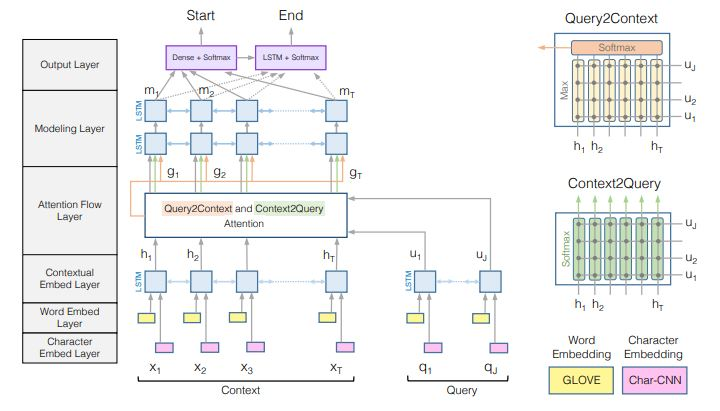
\includegraphics[width=\textwidth,height=8cm]{bidaf_architecture.JPG}
  \caption{Bi-directional attention flow network architecture}
\end{figure*}


%\centering
%

\subsection{Transfer learning}
\label{ssec:transfer_learning}
Here we provide useful definitions and conventions related to transfer learning. Let a domain  $\textbf{D}$ consist of a feature space $\textbf{X}$ and a marfinal probability distribution $P(X)$. Given a source domain $\textbf{D}_s$ and a learning task $\textbf{T}_s$, a target domain $\textbf{D}_t$ and a target task $\textbf{T}_t$, \textit{trasnfer learning} aims to improve the learning of the predictive function for $\textbf{D}_t$ using the knowledge in $\textbf{D}_s$ and $\textbf{T}_s$. In the \textit{inductive transfer learning} setting, the target task is different from the source task, no matter when the source and target domains are the same of not. Conversely, in \textit{transductive transfer learning}, the source and target tasks are the same, while the domains are different. In this situation, little or no labeled data are available in the target domain, while lots of data are present for the source domain \cite{surveytransferlearning} \cite{conneau:2017} \cite{deepcontextualizedwr} \cite{conneau:2017}. 

In computer vision, neural network models are rarely trained from scratch. In general, initial weights are the result of training with ImageNet \cite{imagenet}, a large-scale hierarchical image database, to obtain features. There is already relevant work studying transfer learning over text tasks, mostly around vector representations of words. 

\section{Methods}
\label{sec:methods}

In this section, we describe our methods to study transfer learning over BiDAF networks. 

First, we train a BiDAF network on the SQuAD dataset, being this our source task and domain, and we'll refer to the resulting model as the \textit{source model}. Since we want to study how we can transfer the knowledge to other tasks and domains with none or limited labeled data, we perform a number of transfer experiments with varying amounts of labeled question-answer pairs from the MS-MARCO dataset, which will be our target task and domain for transfer learning.

Let $n$ be the number of labeled samples in the target domain we want to experiment with, then an experiment is as follows: Select $n$ random question-answer pairs from the MS-MARCO dataset, re-train the source model on the randomly selected pairs, and evaluate the resulting model on the MS-MARCO evaluation set. We run this experiment multiple times, for different values of $n$, including $n=0$, which is the case where the target domain has $0$ labeled examples. 

Finally, we also train another BiDAF network on the MS-MARCO dataset without transfer, as a goal for accuracy. The ideal result of this experiment is to achieve similar accuracy in our transfer experiments as in this non-transfer model, which would mean that we can perform this task successfully without fully training our model for this task. It is worth noting that BiDAF performance over MS-MARCO was never studied, but we will compare the results to those 

\section{Results}
\label{sec:results}

\subsection{BiDAF over SQuAD dataset}

The first step of our research is to train a BiDAF over the SQuAD dataset. We train for 16.4 hs using a single NVidia K80 GPU, and obtain near state of the art results, with exact match percentage of $65.64$ and F1 score of $75.68$. The baseline logistic regression performance for this dataset is exact match percentage of $40.0$ and F1 score of $51$. Human performance for this task is EM at $82.3$ and F1 score of $91.2$ \cite{squad:2016} \cite{rnet}.

\subsection{BiDAF over MS-MARCO dataset}

We also consider the baseline models for MS-MARCO dataset. The baseline performance for this dataset using memory networks for passages is ROUGE-L at $0.119$ and BLEU $0.340$ \cite{msmarco:2016}. One of the top results for MS-MARCO, R-NET \cite{rnet}, report ROUGE-L $0.4289$ and BLEU $0.4222$. Human performance was ascertained by having two judges answering the same question and measuring their responses, obtaining ROUGE-L $0.47$ and BLEU $0.46$.


\section{Next steps}
\label{sec:next_steps}

\subsection {BiDAF over MS-MARCO }

The next step to follow in the implementation is to train a BiDAF network over the MS-MARCO dataset. There is a major difference in that the MS-MARCO dataset has multiple text passages for each question, corresponding with the multiple results from the web query. R-NET has achieved the top results in the MS-MARCO leaderboard by concatenating all the candidate passages, which makes the data from MS-MARCO and SQuAD have the same shape. This training involves no transfer, it is used only for comparison with future models.

\subsection {MS-MARCO Evaluation}

While the passages provided in MS-MARCO generally contain useful information for the queries, the answer could contain words outside of the query. Because of the nature of the dataset, the authors of MS-MARCO chose to use ROUGE-L and phrasing-aware evaluation framework to measure performance for long textual answers. We will implement ROUGE-L and BLEU metrics \cite{msmarco:2016}.

\subsection{Transfer experiment}

We will write the transfer experiment where we train a model with SQuAD and then re-train with a different numbers of samples from MS-MARCO (including zero examples). We will then evaluate the obtained accuracy metrics with our non-transfer MS-MARCO model. 




% include your own bib file like this:
%\bibliographystyle{acl}
%\bibliography{acl2018}
\bibliography{acl2018}
\bibliographystyle{acl_natbib}



\end{document}
